\documentclass[10pt,a4paper]{article}
\usepackage[english]{babel}
\usepackage{amsmath}
\usepackage{amsfonts}
\usepackage{graphics}
\usepackage{epsfig}
\usepackage{amssymb}
\usepackage{graphicx}
\author{Elisabeth Lindquist, Fredrik Lundell, Johan Peterson}
\title{\textsc{Deformation of tetrahedral meshes using the Finite Element Method}\\\begin{small}\textsc{Tsbk03 - Advanced game programming}\end{small}}
\begin{document}
\maketitle
\begin{abstract}
%Abstract
In this report we describe the background theory of how the finite element method can be used to deform bodies in a virtual environment as well as presenting how we implemented it. In more detail the mechanics of physical bodies will be brought up, like how stress and strain affects them and results in internal forces which will in turn cause deformations. We will then continue and describe how to discretize the system using the finite element method, bring up and explain the different terms necessary to give a good understanding of the problem. 

Since our goal was to achieve deformations in real time a lot of considerations was taken to linearize several problems. This did not go without the cost of artifacts, so there will be an explanation of how the warped stiffness method proposed by M\"uller is used to compensate for these.
\end{abstract}
\pagebreak
\tableofcontents
\pagebreak

\section{Introduction}
In the real world all materials are deformable in some extent. Even something as solid as a diamond can be deformed using the right amount of force. How to represent the physical properties of an object varies upon the application. It is common to use a rigid body model for simulating a solid object although other methods is needed to capture the inner dynamics of an object. 

There are however simpler methods for simulating deformable objects, such as a mass-spring system. A mass-spring system defines the object as a set of particles interconnected by springs. The behavior of the system depends on how each spring is connected and the number of springs holding the object together. The implementation is straight-forward although there are drawbacks using this method for deforming three dimensional objects.

Our implementation uses the finite element method to solve the problem of deforming three dimensional objects. The finite element method has a long history and where mainly originated from the need of solving complex structural analysis problems in civil engineering. It has successfully been used for stress analysis and this approach is applicable for simulating how a object deformers during stress. 

\subsection{Structure of the report}
This second section of the report first describes some of the terms used in physical body mechanics, and how they relate to deformation of objects. Simplifications to the problem, such as linearization, and the consequences of these are then explained. The third section of the report describes some aspects of the implementation. Results are shown in section four, and discussed in section five. 

\section{Method}

\subsection{Physical body Mechanics}
The elasticity of a material is often expressed with Hook's law approximated as a linear combination of stress and strain\ref{ett}.

\begin{equation}\label{ett}
    \frac{F_{n}}{A} = E \frac{\triangle l}{l}
\end{equation}
External forces acting on a surface gets transmitted through the material causing inner forces a quantity described as stress. This stress acting on a body gives rise to strain an measurement of deformation defined as the relatively elongation or compression of the material.

In one dimension the stress $\sigma$ is a scalar describing the force $ F_{n}$ acting perpendicular to the surface cross-sectional area $A$.
This force causes deformation or strain defined as the difference in length of the material perpendicular to the surface $\triangle A$. Stress and strain is related through Young's modulus $E$ which states the stiffness of the material.

\subsection{Stress and Strain in three dimensions}\label{stressnstrain}
In three dimensions the stress and strain is different depending on the direction of measurement. A point can be strained in one direction and compressed in another thus stress and strain cant be expressed with a single scalar.

A displacement field $\mathbf{u}$ is described as the difference of each points in its initial and deformable state. Hence a point can be strained differently in all direction $\mathbf{u}$ is a vector field described in \ref{tva}.


\begin{eqnarray}\label{tva}
    \mathbf{u}(x, y, z) = \left[ \begin{array}{c}
u(x, y, z) \\
v(x, y, z) \\
w(x, y, z) \end{array} \right]
\end{eqnarray}

The point $x$ new position can be evaluated through the displacement field $p=x+\mathbf{u(x)}$
where $p+dp = x+dx + \mathbf{u(x+dx)} => dp = dx + \mathbf{u(x+dx)}-\mathbf{u(x)} = dx +\nabla \mathbf{u(x)}dx$. Where $\nabla \mathbf{u(x)}$ is the gradient of the displacement field $u$. The strain tensor is a 3x3 matrix and can be derived from the spatial derivatives of the displacement field as illustrated in equation \ref{tre}

\begin{equation}\label{tre}
    \epsilon = \bigtriangledown u + \bigtriangledown u^{T} + \bigtriangledown u^{T} \bigtriangledown u
\end{equation}

This tensor is called Green’s strain tensor and is symmetric and nonlinear. The tensor has the important property of behaving linear for small deformations
and by removing the nonlinear term, Cauchy’s strain tensor is formed. The tensor is illustrated in equation 4 where $\epsilon_{xx}, \epsilon_{yy}, \epsilon_{zz}$ is represents normal strain and $\epsilon_{xy}, \epsilon_{xy}, \epsilon_{xz}$  shear strain.

\begin{eqnarray}\
\epsilon =  \left[ \begin{array}{cccc}
\epsilon_{xx} & \epsilon_{xy} & \epsilon_{xz} \\
\epsilon_{xy} & \epsilon_{yy} & \epsilon_{yz} \\
\epsilon_{xz} & \epsilon_{yz} & \epsilon_{zz} \\
 \end{array} \right]
\end{eqnarray}

In coherency with strain, three dimensional stress also varies in the direction of measurement. As a result, stress is represented as a 3x3 tensor as shown in equation \ref{fem}.

\begin{eqnarray}\label{fem}
\sigma =  \left[ \begin{array}{cccc}
\sigma_{xx} & \sigma_{xy} & \sigma_{xz} \\
\sigma_{xy} & \sigma_{yy} & \sigma_{yz} \\
\sigma_{xz} & \sigma_{yz} & \sigma_{zz} \\
 \end{array} \right]
\end{eqnarray}
Where $\sigma \cdot n = \frac{dF_{n}}{dA}$ gives the stress measuring in direction $n$.

\subsection{Redefine Hook's Law}
Assuming an linear relationship between stress and strain Hooke's law can be redefined as equation \ref{sex}.

\begin{equation}\label{sex}
    \sigma = E \cdot \epsilon
\end{equation}

 $E$ is the connection between stress and strain and depends on properties of the material. For simplicity only isotropic materials is considered, isotropic meaning that the material properties are independent of directions. Material such as plastics or different kinds of alloys are examples of isotropic materials where wood is an example of an anisotropic material which is weaker along rather than across the grains.

Both stress and strain is represented with symmetrical 3x3 tensors. Symmetrical 3x3 matrices only depend on 6 variables hence
$\sigma$ and $\epsilon$ is vectors of dimensionality 6x1. $E$ can then be defined as 6x6 matrix which for isotropic materials only depends on two elastic constants, Young's modulus $E$ and the Poisson's ratio $\nu$. Young's modulus is the ratio of stress or elasticity and Poisson's ratio describes to which amount volume is conserved. Using these notations Hook's law now can be written as equation \ref{eqn:ststhooks} assuming the use of isotropic materials.

\begin{eqnarray}\label{eqn:ststhooks}
\left[ \begin{array}{c}
\epsilon_{xx} \\
\epsilon_{xx} \\
\epsilon_{xx} \\
\epsilon_{xx} \\
\epsilon_{xx} \\
\epsilon_{xx} \\
\end{array} \right] = \frac{E}{(1+\nu)(1-2\nu)}
\left[ \begin{array}{cccccc}
1-\nu & \nu & \nu & 0 & 0 & 0\\
\nu & 1-\nu & \nu & 0 & 0 & 0\\
\nu & \nu & 1-\nu & 0 & 0 & 0\\
0 & 0 & 0 & 1-2\nu & 0 & 0\\
0 & 0 & 0 & 0 & 1-2\nu & 0\\
0 & 0 & 0 & 0 & 0 & 1-2\nu\\
 \end{array} \right]
\left[ \begin{array}{c}
\epsilon_{xx} \\
\epsilon_{xx} \\
\epsilon_{xx} \\
\epsilon_{xx} \\
\epsilon_{xx} \\
\epsilon_{xx} \\
\end{array} \right]
\end{eqnarray}



\subsection{Discretization using Finite element method}
The finite element method (FEM) is a well known numerical method for approximating a solution to a continues problem. The whole domain is sampled into a set of finite elements and as elements volume converges to zero FEM becomes an highly accurate approach for approximating a analytical solution. FEM has been around for decades and is applicable to a wide range of physical and engineering problems such as mechanical, structural and thermal analysis.

\subsubsection{Local stiffness of a tetrahedron element}\label{sec:localstiffness}
The volume of the deformable object is divided into a finite number of linear tetrahedral elements. A tetrahedron is an three dimensional object which has four nodes each having three degrees of freedom, as shown in figure \ref{fig:tetracoord}.

\begin{figure}[htpb]
\centering
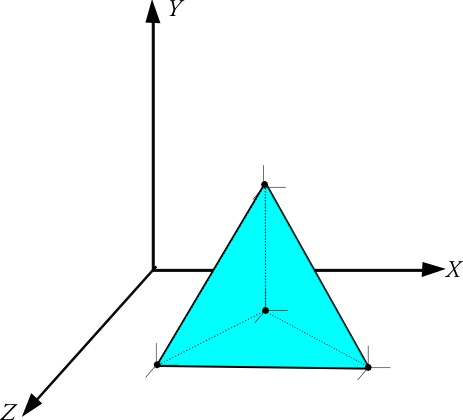
\includegraphics[width=.3\columnwidth]{figures/tetra_coord.png}
\caption{A tetrahedral element with three degrees of freedom per node}
\label{fig:tetracoord}
\end{figure}

The displacement field $u(x,y,z)$ is continues and must be discretisized in order to use the finite element approach. In equation \ref{nio} the displacement field $u(x,y,z)$ is obtained by using $N(x,y,z)$ which is a 12x3 matrix containing the shape functions used to interpolate displacement values inside the tetrahedron. The shape matrix is multiplied with the displacement vector $\hat{u}$ as in \ref{nio}, $\hat{u}$ is a 12x1 vector containing the displacement x,y,z at each node of the tetrahedron. This multiplication gives a approximated displacement field $u(x,y,z)$ which is constant for the whole tetrahedron.

\begin{equation}\label{nio}
    \mathbf{u} \approx N(x,y,z) \hat{u}
\end{equation}

To obtain the strain tensor $\epsilon$ the approximated displacement field is multiplied by L which essential consist of differential operators used to get the partial differential of $u$.

\begin{equation}\label{tio}
    \epsilon = LN \hat{u} = B_ {e} \hat{u}
\end{equation}

$B_ {e}$ is called the strain matrix which is constant and can be precomputed for all elements.

As a result of the strain matrix $B_{e}$ the entire stiffness of the tetrahedron element can be expressed as the stiffness matrix $K_{e}$ connecting all degrees of freedom of a tetrahedron. The stiffness matrix contains information about stress and strain and can analytically be seen as the measures the magnitude of a stress field.

The element stiffness matrix is calculated in equation \ref{eqn:stiffnessmatrix} where $V_{e}$ is the volume of the element and $E$ is the material properties defined in \ref{eqn:ststhooks}.

\begin{equation}\label{eqn:stiffnessmatrix}
    K_{e} = V_{e} B_ {e}^{T}EB_ {e}^{T}
\end{equation}

The element stiffness matrix describes the relationship between all degrees of freedom of a tetrahedron an relates through Hook's law as equation

\begin{equation}\label{eqn:force}
    f_{e} = K_ {e}\hat{u}
\end{equation}

If a node displacement occurs this relationship gives the interconnecting forces accumulated for all node spanning the finite element.

\subsubsection{Global stiffness of a tetrahedron mesh}
For the purpose of a global solution all local stiffness matrices $K_{e}$ is assembled into global stiffness matrix $K$. The assembling process is not trivial and need to be composed in way so that a force affecting one elements deflect the others through the body. How to compose the global stiffness matrix from different types of finite elements etc.

 Since a large part of the dynamics in the global stiffness matrix $K$ is overlapping $K$ tends to be sparse. The dimensionality of $K$ is $3 \cdot n x 3 \cdot n$ where 3 is the degrees of freedom and n is the number of nodes inside the entire object.

\subsubsection{Global system dynamics}
%GlobalSystemDynamics
As presented in M\"uller et al. [1] an elastic object can be simulated by applying Newton's second law of motion $\mathbf{f} = m\ddot{\mathbf{x}}$ on the volymetric elements. Since these elements are infinitesmal and has no mass defined the equation of motion is divided by the volume of the element. Which means that the mass turns to density and the forces turn to body forces. By taking the internal forces into consideration the dynamics that governs the system are described by the following partial differential equation  

\begin{equation}\label{eqn:contPDE}
    \rho \ddot{\bf x} ={\mathbf f}_{ext} + {\mathbf f}_{in}
\end{equation}

Where $\rho$ is the density, ${\mathbf f}_{in}$ are the inner forces caused by stress and ${\mathbf f}_{ext}$ are the external forces. This equation is currently on analytical form and to be able to solve it for an object containing finite elements it can be discretized as

\begin{equation}\label{eqn:discPDE}
\mathbf{M\ddot{x}} + \mathbf{K(x- x_0)} =  \mathbf{f}_{ext}
\end{equation}

However, when working on highly dynamic system where forces are being exerted on solids a damping matrix $\mathbf{C}$ needs to be taken into consideration as described by [fem]. So the system equation can be rewritten as

\begin{equation}\label{eqn:fullDiscPDE}
\mathbf{M\ddot{x}} + \mathbf{C\dot{x}} + \mathbf{K(x-x_0)} =  \mathbf{f}_{ext}
\end{equation}

$\mathbf{M}$ is the mass matrix which is calculated by using nodal quadrature [hans] and $\mathbf{C}$ can be approximated as
\begin{equation}\label{eqn:BuildC}
\mathbf{\mathbf{C}} = \alpha \mathbf{M} + \beta \mathbf{K}
\end{equation}

It is important to note that $\alpha$ and $\beta$ can be found experimentally for different materials.


\subsubsection{Integration}
%Integration
Now that the dynamics of the system are defined we want to be able to integrate over the time domain to actually simulate the deformation. This can be done by either using explicit or implicit integration. Explicit integration has the upside of being easy to implement, however it suffers from being only conditionally stable and the errors accumulate. Implicit integration on the other hand can be slightly harder to work with but is instead unconditionally stable thus recommended for simulating this kind of system. 

Since the dynamic system was described in the previous section, the equation of motion \ref{eqn:fullDiscPDE} can now be applied to the Implicit Euler form as follows [mullerShort]

\begin{equation}\label{eqn:impEuler}
		(\mathbf{M} + \Delta t  \mathbf{C} + \Delta t^2 \mathbf{K})v^{t+1} = \mathbf{M} v - \Delta t (\mathbf{K}(\mathbf{x} - \mathbf{x}_0) +\mathbf{f}_{ext})
\end{equation}

Where the velocity for the next time step $v^{t+1}$ is what needs to be solved. It can be noticed that equation \ref{eqn:impEuler} is in the form of the discrete Poisson equation $\mathbf{Ax=b}$ which means that the inverse of $\mathbf{A}$ has to be computed. Since this is a rather computationally heavy procedure for especially large matrices, it can be a good idea to consider the use of an algorithm that approximates the result of the velocity, like for example the Conjugate Gradient method.

The Conjugate Gradient method is an iterative numerical algorithm that requires the matrix $\mathbf{A}$ in the discrete Poisson equation to be both sparse and symmetrical. Basically what it does is that it takes the equation as input and solves $\mathbf{x}$, thus making it very applicable for this kind of problem.

\subsection{Warped stiffness}
As described in section \ref{stressnstrain} Cauchy’s strain tensor is only valid for small deformations. This is a problem since only large deformations result in visually interesting effects. In section \ref{eqn:stiffnessmatrix} the stiffness matrix is obtained from $V_{e}$, $B_{e}$ and $E$ which are all constant depending on the initial state of the tetrahedron. Due to large deformations during simulation time this stiffness matrix will become unvalued. M\"uller and Gross \cite{muller_ivm} proposed a solution to this problem called Stiffness Warping. This method compensates the error by rotating the deformed tetrahedron back into its original coordinate frame. The rotation is found by forming the matrix A which is the non translation part of the mapping between the two tetrahedrons shown in equation.

\begin{equation}\label{eqn:mappedTetraMatrix}
    \mathbf{A} = [\mathbf{x}_{1}-\mathbf{x}_{0}, \mathbf{x}_{2}-\mathbf{x}_{0}, \mathbf{x}_{3}-\mathbf{x}_{0}][\mathbf{p}_{1}-\mathbf{p}_{0}, \mathbf{p}_{2}-\mathbf{p}_{0}, \mathbf{p}_{3}-\mathbf{p}_{0}]^{-1}
\end{equation}

A Gram-Schmidt method is used to extract the rotation matrix $\mathbf{R}$  from matrix $\mathbf{A}$ , there are several other ways of doing this procedure, however this one is quite simple and works good for this application. As described in \cite{rt_phys} $\mathbf{A}$ the is in the following form

\begin{equation}\label{eqn:transformationAxes}
    A =[\mathbf{a}_0, \mathbf{a}_1,\mathbf{a}_2]
\end{equation}

Where $\mathbf{a}_i$ are the axes of the transformation described in equation \ref{eqn:mappedTetraMatrix}. Note that it is important to ensure that these are normalized and orthogonal to eachother. The three columns of the rotation matrix are finally computed by using the Gram-Schmidt method as follows

\begin{equation}\label{eqn:r0}
    \mathbf{r}_0 = \frac{\mathbf{a}_0}{| \mathbf{a}_0 |}
\end{equation}

\begin{equation}\label{eqn:r1}
    \mathbf{r}_1 = \frac{\mathbf{a}_1 -  \mathbf{r}_0 \cdot \mathbf{a}_1}{| \mathbf{a}_1 -  \mathbf{r}_0 \cdot \mathbf{a}_1 |}
\end{equation}

\begin{equation}\label{eqn:r2}
    \mathbf{r}_2 =  \mathbf{r}_0 \times  \mathbf{r}_1
\end{equation}

The rotation matrix is then assembled as $\mathbf{R}_e =[ \mathbf{r}_0 ,  \mathbf{r}_1 ,  \mathbf{r}_2]$. It should be noted that $\mathbf{r}_2$ is not computed using the Gram-Schmidth method but is instead the cross product of $\mathbf{r}_0$ and  $\mathbf{r}_1$ to ensure a right handed system.

Now that the rotational part $\mathbf{R}_e$ is extracted from the deformation it can be used to rotate the deformed vertices $\mathbf{x}$ back to their non-rotated state $\mathbf{R}_e^{-1} \mathbf{x}$. By multiplying the displacements in this state with the stiffness matrix $\mathbf{K}_e$ the linear forces $\mathbf{K}_e (\mathbf{R}_e^{-1} \mathbf{x} - \mathbf{x}_0)$ is achieved. These forces are then finally rotated back to the actual deformed state as follows

\begin{equation}\label{eqn:f_warped}
     \mathbf{f}_{warped} = \mathbf{R}_e \mathbf{K}_e (\mathbf{R}_e^{-1} \mathbf{x} - \mathbf{x}_0)
\end{equation}

With this new inner force the global stiffness matrix $\mathbf{K}$ have to be constructed a bit differently by assembling it with $\mathbf{K}'_e = \mathbf{R}_e \mathbf{K}_e \mathbf{R}_e^T$ instead of only $\mathbf{K}_e$. And the implicit euler equation \ref{eqn:impEuler} has to be rewritten as

\begin{equation}\label{eqn:warpedImpEuler}
		(\mathbf{M} + \Delta t  \mathbf{C} + \Delta t^2 \mathbf{K})v^{t+1} = \mathbf{M} v - \Delta t (\mathbf{Kx}-\mathbf{f}_0 + \mathbf{f}_{ext})
\end{equation}

Where 

\begin{equation}\label{eqn:f0}
		\mathbf{f}_0 = \mathbf{R}_e \mathbf{K}_e \mathbf{x}_0
\end{equation}



\begin{figure}[h]
\centering
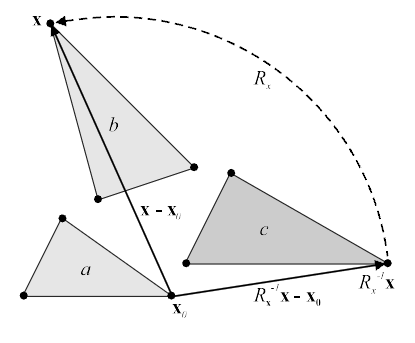
\includegraphics[width=.5\columnwidth]{figures/warpedstiffness.png}
\caption{}
\label{fig:4}
\end{figure}


\subsection{Fracturing}
If the stress on an object is larger than a limit decided by the material properties, the object will not only deform, it will also break. If a fracture is to take place it has to be determined where to break the structure. The method used to determine how the elements break is based on a method by O'Brien and Hodgins \cite{fracture} .

This method calculates a stress tensor $\sigma$ for each element. The stress tensor is calculated in equation \ref{stresser}.
 
 \begin{equation}\label{stresser}
 \sigma = EB_{e}\hat{u}
 \end{equation}
 
 A random node in the element is selected a plane is chosen, and the largest eigenvalue of the stress tensor is used to create a plane through that node. The normal of the plane is set to be the eigenvector corresponding to the largest eigenvalue. All elements that share that node are then found, and they are set to belong to the side of the plane where their center of mass is located, as shown in figure \ref{fig:fracture}. The fracture is then created by inserting new nodes and updating the data structure.

\begin{figure}[htbp]
\label{fig:fracture}
\begin{center}
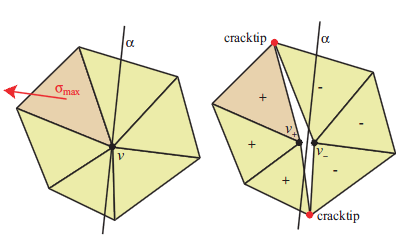
\includegraphics[scale = 0.6]{figures/fracture.png}
\caption{Fracture of nodes}
\end{center}
\end{figure} 


\section{Implementation}
Our application consists of classes divided into three main groups: Representation and creation of tetrahedral meshes, solving the dynamic system and displaying the results. The implementation uses the OpenGL graphics library to render tshe graphics, and the armadillo linear algebra library for performing calculations on vectors and matrices. A graphical user interface is created using the AntTweakBar library.

\subsection{Tetrahedron mesh}
When using the FEM in a volume application, such as ours, a mesh of tetrahedral objects is used. This mesh need to be generated and stored in a suitable data structure.

\subsubsection{Volume generation}
The finite volume elements can be generated in several ways. To create a tetrahedral mesh from a triangle mesh different triangulation methods can be applied. Snice this problem is not the main focus of the project already created tetrahedral objects are used. These are defined as two lists, one containing all vertex points in the tetrahedrons and one containing a list of which vertices that belong to each tetrahedron.

The vertex positions are read from the file and temporarily stored. For each tetrahedron in the tetrahedron list the corresponding vertex indices are found, the positions read and a tetrahedron object is created using these position. The vertices must be placed in an order that results in a tetrahedron with a positive volume. The function for creating a tetrahedron calculates the volume and if it is negative it makes a recursive call with the vertices in a different order.

We have defined the positions and vertex indices of a cube consisting of five tetrahedrons, and also tested our application using some of the meshes created by M\"uller-Fischer \cite{meshes}.


\subsubsection{Data structure}
In order to access the data in efficient way it must be stored in a suitable data structure. We have implemented a data structure consisting of the classes \texttt{Vertex}, \texttt{Face}, \texttt{HalfEdge}, \texttt{Tetrahed} and \texttt{TetrahedMesh}. This structure was inspired by the Compact Half-Face data structure introduced by Lage et al. \cite{halfface}, which has features that makes it possible to optimize for things such as execution speed and memory consumption. We have, however, decided to implement only the parts of the data structure that we have found to be necessary for our application. We have also made some simplifications and changes, where we have favored ease of use with our methods over speed and memory consumption.

\subsubsection{Primitives}
The primitives of a tetrahedral mesh are used to store vertex positions and keeping track of information such as adjacency and face normals. The \texttt{Vertex} class contains functions for setting and retrieving vertex positions. A \texttt{Vertex} also belongs to a \texttt{HalfEdge}, and the corresponding \texttt{HalfEdge} is stored for each \texttt{Vertex}. The \texttt{HalfEdge} class contains functionality for traversing the data structure by keeping the indices of its \texttt{next}, \texttt{prev} and \texttt{pair} \texttt{HalfEdge}. Its functionality is similar to the Half Edge data structure for triangular meshes described by Botsch et al. \cite{Botsch}. The structure is shown in figure \ref{fig:tetraedge}. Each \texttt{HalfEdge} has a \texttt{Face} related to it, and keeps the corresponding index. The \texttt{Face} class also keeps track of which \texttt{Face} belong to which \texttt{HalfEdge}. A \texttt{Face} also has a normal, that can be set and retrieved. It also keeps the indices of its opposite \texttt{Face}. This structure is shown in figure \ref{fig:tetraface}. A tetrahedron is represented by the \texttt{Tetrahed} class, which keeps the indices of a \texttt{Vertex}, a \texttt{HalfEdge} and four \texttt{Faces}.


\begin{figure}[htbp]
\label{fig:tetraedge}
\begin{center}
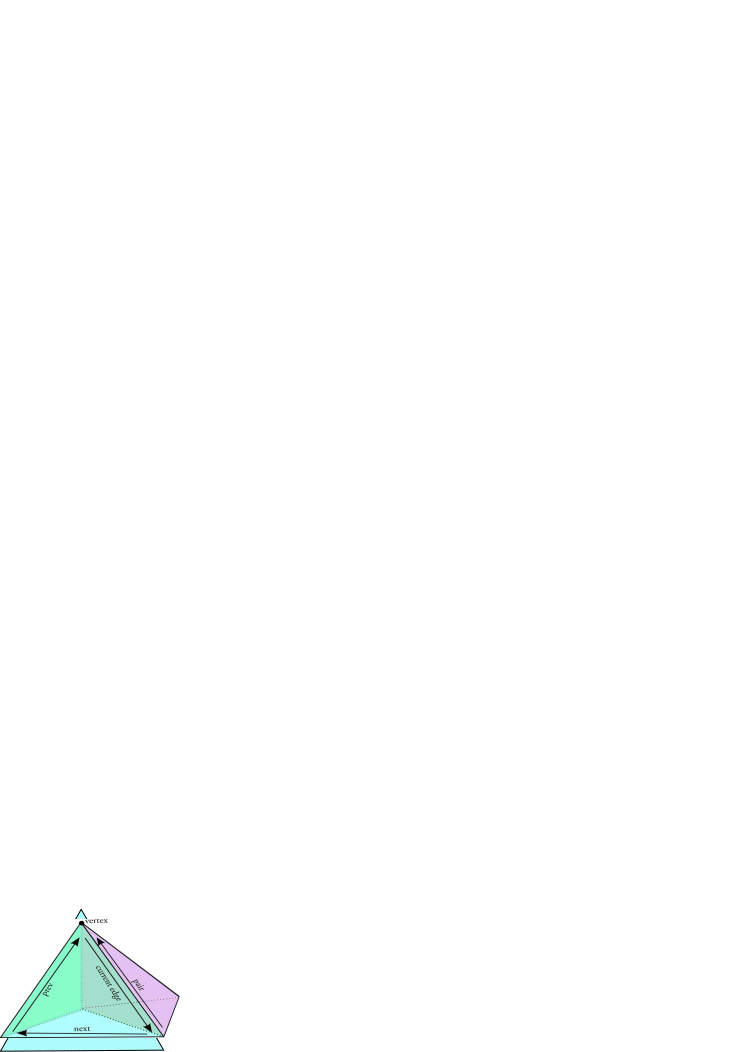
\includegraphics[scale=1]{figures/tetra_edge}
\caption{The Half Edges of a face.}
\end{center}
\end{figure}

\begin{figure}[htbp]
\label{fig:tetraface}
\begin{center}
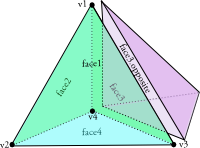
\includegraphics[scale=1]{figures/tetra_face}
\caption{The faces of a tetrahedron.}
\end{center}
\end{figure}


\subsubsection{The \texttt{TetrahedMesh} class}
The \texttt{TetrahedMesh} class contains functions for creating, changing and rendering a tetrahedral mesh. Tetrahedrons are added by creating their primitives, and storing indices of the primitives that make up a tetrahedron. Several modes for rendering are supported, such as the option of rendering normals, edges or faces. 

\subsection{The \texttt{Solver} class}
\subsubsection{Main functionality}
The \texttt{Solver} class contains the functionality for finding a solution to the dynamic
\subsubsection{Constructing the elementwise stiffness matrix}
\subsection{Assembling the global stiffness matrix}
\subsubsection{Conjugate gradient solver}



\section{Results}
\subsection{Images}

\subsection{Performance}

\section{Discussion}
We have created an application that handles deformation of objects with different shapes and material properties. 
\subsection{Improvements and further work}
Although our application is able to perform most of the things we initially had planned, there are of course several improvements that could be made outside the scope of this project. The model itself is simplified, since we use several linearizations. This is partly handled by the introduction of warped stiffness. A more intelligent data structure could be used in order to allow for larger meshes, and parallelization should be utilized in order to ensure real time performance with more complex meshes. 
\subsubsection{Solution on the GPU}
An interesting extension to the implementation would be to execute some tasks in parallel on the GPU. There are sections in the implementation that could probably be well suited for parallelization, such as the conjugate gradient solver. In order to utilize the parallel properties of the GPU the problem must be rewritten. Bolz et al. \cite{gpu} suggests a method for implementing the conjugate gradient method on the GPU that consists of two tasks, computing the sparse matrix-vector multiplication and a vector inner product.

This method makes use of several textures, two containing the non-zero elements of the matrix $\mathbf{A}$ used in the conjugate gradient method, others containing various pointers to indices that makes it possible to know which elements are used . Implementing this method 





\pagebreak
\addcontentsline{toc}{section}{References}
\bibliographystyle{plain}
\bibliography{refs}
\end{document} 